\documentclass[11pt, letterpaper]{article}
\usepackage{graphicx}
\usepackage[export]{adjustbox}
\usepackage{hyperref}
\usepackage{xcolor}
\graphicspath{{images/}}
\usepackage[a4paper, total={6in, 8in}]{geometry}
\usepackage{tabularx}
\usepackage{float}


\title{\textbf {Audio classification with machine learning} \\ \large Introduction to Machine Learning 2024/2025Z}

\author{Łukasz Górski \\ Piotr Iśtok \\ Piotr Jacak \\ Stanisław Janowicz \\ Marcin Falkowski}

\date{Styczeń 2025}


\begin{document}
\maketitle

\newpage
\tableofcontents
\newpage

\section{Abstract}

The task we will be attempting to solve in this project is a binary recognition problem, meaning that the program's main function is to transform a given input into either 1 or 0, depending on certain properties and conditions. Specifically, the input will consist of a single audio file, either uploaded directly or recorded on a recorder with a microphone by the program. We will transform this audio file into a spectrogram and, after cleaning and pre-processing, pass it into the model to determine its membership in class one, representing the people who are granted access, or class zero, or the people who are denied.

The intended use of this project is on a voice-based intercom device that must discern whether a person has the authority to enter restricted areas.

\section{Introduction}

In this section we present some useful background information on audio classification and on the more technical aspects of the project.

\subsection{Audio Classification}
 Audio classification is a machine learning task that involves identifying and tagging audio signals into different classes or categories. In our case, this is done through the analysis of spectrograms of the files provided, since analysis of images is used much more frequently in the field of machine learning.

 Our data set is the \href{https://www.kaggle.com/datasets/psyreddy07/daps-data}{DAPS} set, consisting of .wav files of 20 speakers reading 5 scripts each, averaging at about 14 and a half minutes.

 Of those 20 speakers, F1, F7, F8, M3, M6, M8, are chosen as class 1, and the other speakers form class 0.

 \subsection{Convolutional Neural Networks}
 The model used is a Convolutional Neural Network (CNN), which is a common type of deep learning network employed in tasks of recognition, especially image processing. It consists of an input layer, a number of hidden layers, and an output layer. In our program, the output layer is binary, since we only have 2 classes.

 We chose the \verb|pytorch| library to implement our model.

\section{Methodology}
\section{Exploratory Data Analysis}

Exploratory Data Analysis (or EDA for short) is the process of gathering information from the given data set before using it for the purposes of informed decision making later on. Since our data are in the form of .wav files, we use the \verb | scipy.io.wavfile |Python library to load it in order to analyze it by looking directly at the array representing it. This was our first attempt at EDA, and although the code itself runs quick, it gives us very little useful information. Namely, we only have access to the numbers: the minimum and maximum values of the array, the means, sample rates and the lengths of the files in each class. This is hardly enough - the length of an audio doesn't, and shouldn't, affect how is it classified.

Therefore, we make use of Python libraries that are more suited to accomplishing our goals. After presenting the audio in the form of spectrograms, we extract helpful details into a .csv file, which becomes the input of the next stages of EDA. The details shown in the .csv vary greatly from the simple values of the previous step and are of much greater importance to us. Here are the features that we managed to extract in this way: Person, sex, script, audio type, is a test set, class, and contrast. Let us explain them one by one:
\begin{itemize}
    \item Person - the person speaking in the audio, as described in the Data section,
    \item Gender - the gender of the person (either male or female),
    \item Script - the script read in the audio,
    \item Audio Type - type of audio (either cleanraw, ipadflat, ipad, or iphone)
    \item Is Test Set - a binary value describing whether the file was used in training the model or testing it,
    \item Class - 0 or 1, as described in the Introduction
    \item Contrast - the contrast of the image.
\end{itemize}
Besides these values, there were five other features - average RGB values of the image as well as the Brightness and Saturation. However, as discussed in the Spectrograms section, the spectrograms were in grayscale, making all of these values equal to each other, and thus redundant. Because of this, we have decided to analyze only the mean redness value of the images with the understanding that it also signifies the other features from this section.

With this data, we can begin presenting the previously-numerical information visually, which makes the insights much more obvious to a human observer. We make use of the \verb|seaborn| library to generate histograms like the following:

\begin{figure}[H]
    \centering
    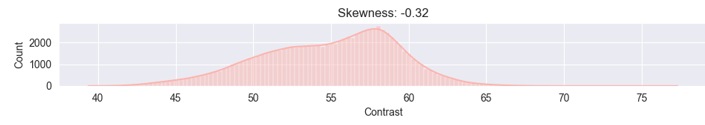
\includegraphics[width=1\linewidth]{image.png}
    \caption{Contrast distribution}
    \label{fig:enter-label}
\end{figure}

We can than utilize the same library to plot pairwise relationships in the data set, checking to what degree two variables are correlated with each other. Using the \verb|heatmap| function, we get the following result:

\begin{figure}[H]
    \centering
    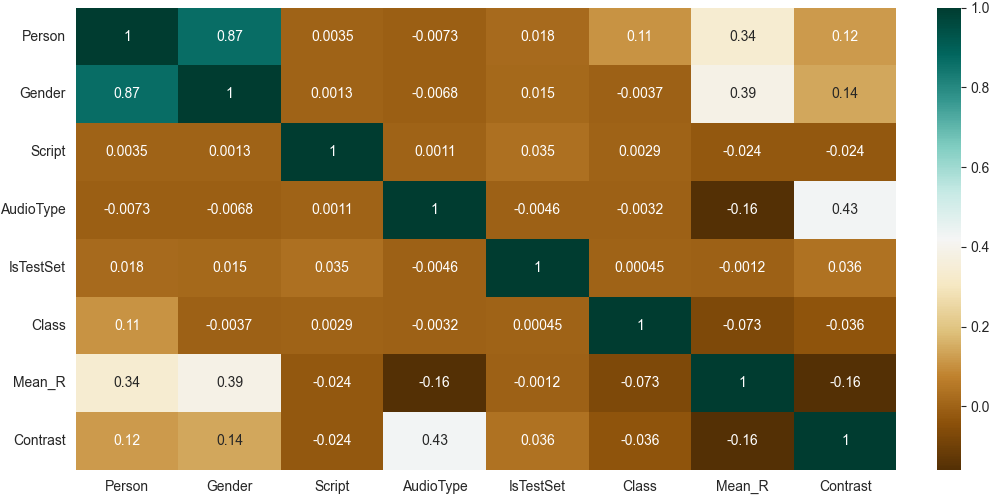
\includegraphics[width=1\linewidth]{pairplot.png}
    \caption{Pairwise relationships in the data set}
    \label{fig:enter-label}
\end{figure}

Lower values indicate a negative correlation between two variables, while values closer to 1 mean a positive association. From this heatmap, we can conclude that the Gender and Person variables are correlated, which means that the data set isn't split evenly between male and female recordings. This is a valuable insight, since it might affect model - if we chose the training set from the original data at random, the model might be worse at classifying one gender than the other.

Fortunately, looking at the value of the intersection between Gender and IsTestSet (0.015), the test set itself is fairly balanced.

\section{Cleaning and pre-processing}
\section{Models used}
\section{Results}

\end{document}